\documentclass{beamer}
\usetheme{Warsaw}

\usepackage[utf8]{inputenc}
\usepackage{fancybox}
\usepackage{multimedia} 
\usepackage{subfig}
\usepackage{amsmath}
\usepackage{hyperref}
\usepackage[all]{xy}
\begin{document}


\title[Stochastik] % (optional, only for long titles)
{Stochastik für Informatiker
\\
\includegraphics[scale=0.5]{img/craps}
}
\subtitle{}
\author[Dr. Johannes Riesterer] % (optional, for multiple authors)
{Dr.  rer. nat. Johannes Riesterer}

\date[KPT 2004] % (optional)
{}

\subject{Stochastik}

\frame{\titlepage}


\begin{frame}
    \frametitle{Allgemeine Wahrscheinlichkeitsräume}
\framesubtitle{}

\begin{block}{Eigenschaften}
Sind $X,Y : \Omega \to \mathbb{R}$   reelle, integrierbare  Zufallsvariablen und $a,b \in \mathbb{R}$ konstant, so gilt:
\begin{align*}
& \mathbb{E}(a \cdot X + b \cdot Y) = a \cdot \mathbb{E}(X) + b \cdot \mathbb{E}(Y) \\
& X(x) \leq Y(x) \;  \forall x \in \Omega \Rightarrow \mathbb{E}(X) \leq \mathbb{E}(Y) \\
& X ,Y \text{ stoch. unabhängig} \Rightarrow   \mathbb{E}(X \cdot Y) =  \mathbb{E}(X) \cdot  \mathbb{E}(Y) \\
& \mathbb{E} (1_A) = P (A)
\end{align*}
\end{block}

 \end{frame}

\begin{frame}
    \frametitle{Allgemeine Wahrscheinlichkeitsräume}
\framesubtitle{}

\begin{block}{Markov-Ungleichung }
Sei $Y : \Omega \to \mathbb{R}$  eine  reelle, integrierbare  Zufallsvariablen und $f : [0, \infty) \to [0, \infty)$ monoton wachsend.
Dann gilt für alle $\epsilon > 0$ mit $f(\epsilon) > 0$
\begin{align*}
P (|Y |  \geq \epsilon) \leq \frac{\mathbb{E} (f \circ |Y|)}{f(\epsilon)}
\end{align*}
\end{block}
\begin{block}{Beweis}
Da $f(\epsilon) 1_{\{ |Y| \geq  \epsilon \} } \leq f \circ |Y|$ folgt
\begin{align*}
f(\epsilon) P(|Y| \geq \epsilon) = & f(\epsilon) \mathbb{E}(1_{\{ |Y| \geq  \epsilon \} }) = \mathbb{E}( f(\epsilon) 1_{\{ |Y| \geq  \epsilon \} }) \\
\leq & \mathbb{E}( f \circ |Y|)
\end{align*}
\end{block}
 \end{frame}


\begin{frame}
    \frametitle{Allgemeine Wahrscheinlichkeitsräume}
\framesubtitle{}

\begin{block}{Varianz}
Die Varianz ist definiert durch
\begin{align*}
\mathbb{V}(X) :=\mathbb{E} \bigl( (X - \mathbb{E}(X))^2 \bigr)
\end{align*}
\end{block}

\begin{block}{Verschiebungssatz}
\begin{align*}
 \mathbb{V}(X) & = \mathbb{E}(X^2 - 2X \mathbb{E}(X) + \mathbb{E}(X)^2) = \mathbb{E}(X^2) - 2 \mathbb{E}(X)^2 +  \mathbb{E}(X)^2 \\
& =  \mathbb{E}(X^2) -  \mathbb{E}(X)^2 \\
\end{align*}
\end{block}
\begin{block}{Eigenschaft (Übung)} 
Für $a,b \in \mathbb{R}$ ist $\mathbb{V}(aX + b)  = a^2   \mathbb{V}(X)$.
\end{block}

 \end{frame}

\begin{frame}
    \frametitle{Allgemeine Wahrscheinlichkeitsräume}
\framesubtitle{}

\begin{block}{Beispiel}
Normalverteilung. $ f(x) = \frac 1{\sigma \sqrt{2\pi}}e^{- \frac {1}{2} (\frac{x- \mu}{ \sigma})^2}$ mit $\mu \in \mathbb{R}, \sigma > 0 $.
\begin{align*}
P_f (A) := \int_{A}  \frac 1{\sigma \sqrt{2\pi}}e^{- \frac {1}{2} (\frac{x- \mu}{ \sigma})^2}dx
\end{align*}
$X: \mathbb{R} \to \mathbb{R} ; X(x) = x$.
\begin{align*}
& \frac{1}{\sqrt{2 \pi}} \int_{- \infty}^{\infty} x (xe^{- \frac{x^2}{2}}) \; dx \\
& =  \frac{1}{\sqrt{2 \pi}} \biggl (\biggl [ x (e^{- \frac{x^2}{2}}) \biggr]_{- \infty}^{\infty}   - \int_{- \infty}^{\infty}  - e^{- \frac{x^2}{2}} \; dx  \biggr) = 0 + 1 = 1\\
\end{align*}
\href{https://de.wikipedia.org/wiki/Partielle_Integration}{LINK: Partielle Integration}. Mit Folien vom letzten mal über $\mathbb{E}(X)$
$\Rightarrow \mathbb{V}(X) = \sigma^2$.
\end{block}

 \end{frame}





\begin{frame}
    \frametitle{Allgemeine Wahrscheinlichkeitsräume}
\framesubtitle{}

\begin{block}{Tschebyscheff-Ungleichung }
Für eine  eine  reelle, integrierbare und quadratintegrierbare  Zufallsvariablen $Y : \Omega \to \mathbb{R}$  gilt:
\begin{align*}
P (|Y  - \mathbb{E} (Y)|  \geq \epsilon) \leq \frac{\mathbb{V} (Y)}{ \epsilon^2} 
\end{align*}
\end{block}
\begin{block}{Beweis}
Folgt direkt aus der Markov-Ungleichung mit $Y' = Y -\mathbb{E}(Y)$ und $f(x) = x^2$
\end{block}
 \end{frame}



\begin{frame}
    \frametitle{Allgemeine Wahrscheinlichkeitsräume}
\framesubtitle{}

\begin{block}{Schwaches Gesetzt der großen Zahlen }
Seien $\{X_i  \}_i: \Omega \to \mathbb{R}$ unabhängige, reelle Zufallsvariablen (uid, iid(englisch)) mit $\mathbb{E}(X_i) = \mu < \infty$ und $\mathbb{V}(X_i) = \sigma < \infty$, dann gilt
\begin{align*}
P \bigl  ( \bigl | \frac{1}{n} \sum_{i=1}^{n} X_i - \mu \bigr |  \geq \epsilon \bigr) \leq \frac{\sigma}{ n \cdot \epsilon^2} \; \; \underset{n \to \infty}{\longrightarrow} 0
\end{align*}
(stochastische Konvergenz). 
\end{block}
\begin{block}{Beweis}
Mit $Y_n =  \frac{1}{n} \sum_{i=1}^{n}  X_i - \mu$ ist $\mathbb{E}(Y_n) =  \frac{1}{n} \sum_{i=1}^{n} \mathbb{E}( X_i - \mu) = 0$ und 
$\mathbb{V}(Y_n) =  \frac{1}{n^2} \sum_{i=1}^{n} \mathbb{V}( X_i ) = \frac{\sigma}{n}$. Aus der Tschebyscheff-Ungleichung folgt die Behauptung.
\end{block}
 \end{frame}


\begin{frame}
    \frametitle{Allgemeine Wahrscheinlichkeitsräume}
\framesubtitle{}

\begin{block}{Schwaches Gesetzt der großen Zahlen }
Konvergenz in Wahrscheinlichkeit macht keine Aussage über die Qualität der Konvergenz über die Laufzeit hinweg.
\end{block}
\begin{figure}[htp]
      \centering
    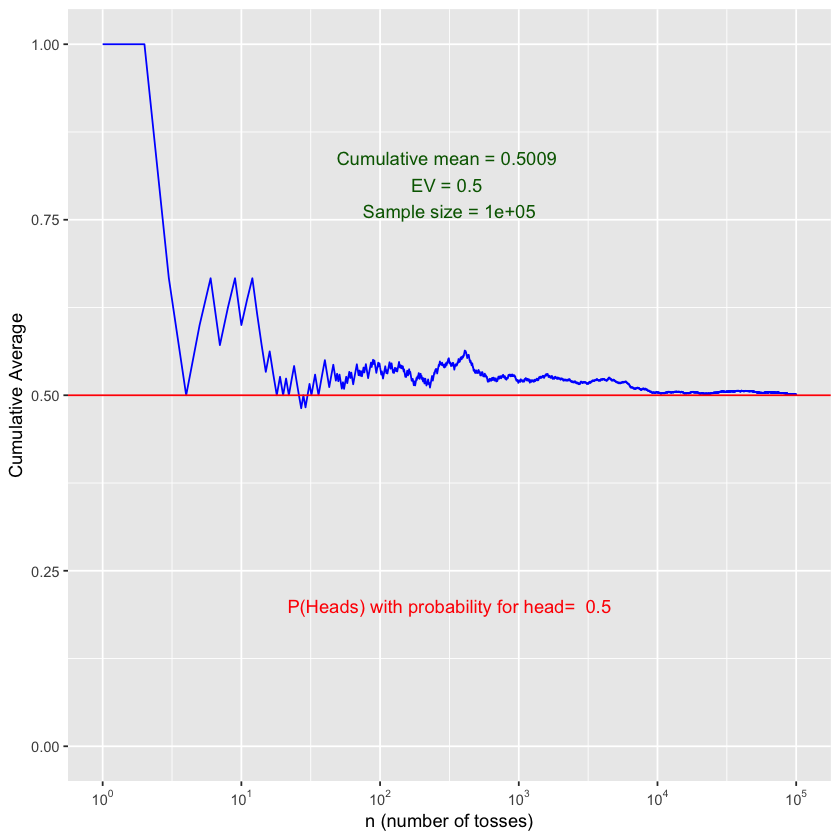
\includegraphics[width=0.55\textwidth]{img/lln}
      \caption{Quelle: Wikipedia}
\end{figure}


 \end{frame}


\begin{frame}
    \frametitle{Allgemeine Wahrscheinlichkeitsräume}
\framesubtitle{}

\begin{block}{Fast sichere Konvergenz}
Fast sicher
\begin{align*}
P \bigl  ( \omega \in \Omega : Y_n (\omega)\to Y(\omega) \bigr) = 1
\end{align*}
$Y_n$ konvergiert fast überall gegen $Y$ für $n \to \infty$. Der Fehler wird mit wachsendem $n$ kleiner (bis auf Nullmenge)

\end{block}
\begin{block}{starkes Gesetzt der großen Zahlen }
\begin{align*}
\frac{1}{n} \sum_n (X_i) \underset{n \to \infty}{\longrightarrow} \mu \text { fast sicher}
\end{align*}
\end{block}

 \end{frame}


\end{document}
